\documentclass{article}

\usepackage{booktabs}
\usepackage{fancyhdr}
\usepackage{float}
\usepackage{graphicx}
\usepackage{helvet}
\usepackage{hyperref}
\usepackage{tabularx}
\usepackage{xcolor}

\usepackage{listings}
\usepackage{tikz}

\usepackage{makeidx}         % allows index generation
\makeindex

\lstset{frame=tblr,
  rulecolor=\color{lightgray},
  language=Java,
  aboveskip=5mm,
  belowskip=5mm,
  showstringspaces=false,
  columns=flexible,
  basicstyle=\linespread{1.0}\small\ttfamily,
  numbers=none,
  % numberstyle=\tiny\color{gray},
  % keywordstyle=\color{blue},
  % commentstyle=\color{dkgreen},
  % stringstyle=\color{mauve},
  breaklines=true,
  breakatwhitespace=true,
  tabsize=3
}

\usepackage{framed}     % These needed for the code formatter
\usepackage{color}
\usepackage{fancyvrb}

% Use helvetica (sans) by default
\renewcommand{\familydefault}{\sfdefault}

% Greenish links
\hypersetup{
  colorlinks=true,
  linkcolor=blue!50!red,
  urlcolor=blue!50!red
}

\setlength{\headheight}{40pt}
\setlength{\headsep}{0.2in}

\pagestyle{fancy}
\lhead{
\includegraphics[width=0.2\textwidth]{img/logo}}
\chead{SPIDriver User Guide}
\rhead{\thepage}
\cfoot{\textcopyright \the\year \ \ Excamera Labs}
\renewcommand{\headrulewidth}{0.5pt}
\renewcommand{\footrulewidth}{0.5pt}

\usepackage{array}
\newcolumntype{L}[1]{>{\raggedright\let\newline\\\arraybackslash\hspace{0pt}}m{#1}}
\newcolumntype{C}[1]{>{\centering\let\newline\\\arraybackslash\hspace{0pt}}m{#1}}
\newcolumntype{R}[1]{>{\raggedleft\let\newline\\\arraybackslash\hspace{0pt}}m{#1}}

\usepackage{setspace}

\newcommand{\heavyline}{\specialrule{1pt}{1pt}{1pt}}
\newcommand{\png}[1]{
\begin{figure}[H]
\begin{center}
\includegraphics[width=0.75\textwidth]{#1}
\end{center}
\end{figure}
}
\newcommand{\pngw}[2]{
\begin{figure}[H]
\begin{center}
\includegraphics[width=#2\textwidth]{#1}
\end{center}
\end{figure}
}

\newcommand{\mach}[1]{\texttt{\textbf{#1}}}
\newcommand{\gap}{\vspace{10pt}}


\makeatletter
\def\PY@reset{\let\PY@it=\relax \let\PY@bf=\relax%
    \let\PY@ul=\relax \let\PY@tc=\relax%
    \let\PY@bc=\relax \let\PY@ff=\relax}
\def\PY@tok#1{\csname PY@tok@#1\endcsname}
\def\PY@toks#1+{\ifx\relax#1\empty\else%
    \PY@tok{#1}\expandafter\PY@toks\fi}
\def\PY@do#1{\PY@bc{\PY@tc{\PY@ul{%
    \PY@it{\PY@bf{\PY@ff{#1}}}}}}}
\def\PY#1#2{\PY@reset\PY@toks#1+\relax+\PY@do{#2}}

\expandafter\def\csname PY@tok@gd\endcsname{\def\PY@tc##1{\textcolor[rgb]{0.63,0.00,0.00}{##1}}}
\expandafter\def\csname PY@tok@gu\endcsname{\let\PY@bf=\textbf\def\PY@tc##1{\textcolor[rgb]{0.50,0.00,0.50}{##1}}}
\expandafter\def\csname PY@tok@gt\endcsname{\def\PY@tc##1{\textcolor[rgb]{0.00,0.27,0.87}{##1}}}
\expandafter\def\csname PY@tok@gs\endcsname{\let\PY@bf=\textbf}
\expandafter\def\csname PY@tok@gr\endcsname{\def\PY@tc##1{\textcolor[rgb]{1.00,0.00,0.00}{##1}}}
\expandafter\def\csname PY@tok@cm\endcsname{\let\PY@it=\textit\def\PY@tc##1{\textcolor[rgb]{0.25,0.50,0.50}{##1}}}
\expandafter\def\csname PY@tok@vg\endcsname{\def\PY@tc##1{\textcolor[rgb]{0.10,0.09,0.49}{##1}}}
\expandafter\def\csname PY@tok@m\endcsname{\def\PY@tc##1{\textcolor[rgb]{0.40,0.40,0.40}{##1}}}
\expandafter\def\csname PY@tok@mh\endcsname{\def\PY@tc##1{\textcolor[rgb]{0.40,0.40,0.40}{##1}}}
\expandafter\def\csname PY@tok@go\endcsname{\def\PY@tc##1{\textcolor[rgb]{0.53,0.53,0.53}{##1}}}
\expandafter\def\csname PY@tok@ge\endcsname{\let\PY@it=\textit}
\expandafter\def\csname PY@tok@vc\endcsname{\def\PY@tc##1{\textcolor[rgb]{0.10,0.09,0.49}{##1}}}
\expandafter\def\csname PY@tok@il\endcsname{\def\PY@tc##1{\textcolor[rgb]{0.40,0.40,0.40}{##1}}}
\expandafter\def\csname PY@tok@cs\endcsname{\let\PY@it=\textit\def\PY@tc##1{\textcolor[rgb]{0.25,0.50,0.50}{##1}}}
\expandafter\def\csname PY@tok@cp\endcsname{\def\PY@tc##1{\textcolor[rgb]{0.74,0.48,0.00}{##1}}}
\expandafter\def\csname PY@tok@gi\endcsname{\def\PY@tc##1{\textcolor[rgb]{0.00,0.63,0.00}{##1}}}
\expandafter\def\csname PY@tok@gh\endcsname{\let\PY@bf=\textbf\def\PY@tc##1{\textcolor[rgb]{0.00,0.00,0.50}{##1}}}
\expandafter\def\csname PY@tok@ni\endcsname{\let\PY@bf=\textbf\def\PY@tc##1{\textcolor[rgb]{0.60,0.60,0.60}{##1}}}
\expandafter\def\csname PY@tok@nl\endcsname{\def\PY@tc##1{\textcolor[rgb]{0.63,0.63,0.00}{##1}}}
\expandafter\def\csname PY@tok@nn\endcsname{\let\PY@bf=\textbf\def\PY@tc##1{\textcolor[rgb]{0.00,0.00,1.00}{##1}}}
\expandafter\def\csname PY@tok@no\endcsname{\def\PY@tc##1{\textcolor[rgb]{0.53,0.00,0.00}{##1}}}
\expandafter\def\csname PY@tok@na\endcsname{\def\PY@tc##1{\textcolor[rgb]{0.49,0.56,0.16}{##1}}}
\expandafter\def\csname PY@tok@nb\endcsname{\def\PY@tc##1{\textcolor[rgb]{0.00,0.50,0.00}{##1}}}
\expandafter\def\csname PY@tok@nc\endcsname{\let\PY@bf=\textbf\def\PY@tc##1{\textcolor[rgb]{0.00,0.00,1.00}{##1}}}
\expandafter\def\csname PY@tok@nd\endcsname{\def\PY@tc##1{\textcolor[rgb]{0.67,0.13,1.00}{##1}}}
\expandafter\def\csname PY@tok@ne\endcsname{\let\PY@bf=\textbf\def\PY@tc##1{\textcolor[rgb]{0.82,0.25,0.23}{##1}}}
\expandafter\def\csname PY@tok@nf\endcsname{\def\PY@tc##1{\textcolor[rgb]{0.00,0.00,1.00}{##1}}}
\expandafter\def\csname PY@tok@si\endcsname{\let\PY@bf=\textbf\def\PY@tc##1{\textcolor[rgb]{0.73,0.40,0.53}{##1}}}
\expandafter\def\csname PY@tok@s2\endcsname{\def\PY@tc##1{\textcolor[rgb]{0.73,0.13,0.13}{##1}}}
\expandafter\def\csname PY@tok@vi\endcsname{\def\PY@tc##1{\textcolor[rgb]{0.10,0.09,0.49}{##1}}}
\expandafter\def\csname PY@tok@nt\endcsname{\let\PY@bf=\textbf\def\PY@tc##1{\textcolor[rgb]{0.00,0.50,0.00}{##1}}}
\expandafter\def\csname PY@tok@nv\endcsname{\def\PY@tc##1{\textcolor[rgb]{0.10,0.09,0.49}{##1}}}
\expandafter\def\csname PY@tok@s1\endcsname{\def\PY@tc##1{\textcolor[rgb]{0.73,0.13,0.13}{##1}}}
\expandafter\def\csname PY@tok@sh\endcsname{\def\PY@tc##1{\textcolor[rgb]{0.73,0.13,0.13}{##1}}}
\expandafter\def\csname PY@tok@sc\endcsname{\def\PY@tc##1{\textcolor[rgb]{0.73,0.13,0.13}{##1}}}
\expandafter\def\csname PY@tok@sx\endcsname{\def\PY@tc##1{\textcolor[rgb]{0.00,0.50,0.00}{##1}}}
\expandafter\def\csname PY@tok@bp\endcsname{\def\PY@tc##1{\textcolor[rgb]{0.00,0.50,0.00}{##1}}}
\expandafter\def\csname PY@tok@c1\endcsname{\let\PY@it=\textit\def\PY@tc##1{\textcolor[rgb]{0.25,0.50,0.50}{##1}}}
\expandafter\def\csname PY@tok@kc\endcsname{\let\PY@bf=\textbf\def\PY@tc##1{\textcolor[rgb]{0.00,0.50,0.00}{##1}}}
\expandafter\def\csname PY@tok@c\endcsname{\let\PY@it=\textit\def\PY@tc##1{\textcolor[rgb]{0.25,0.50,0.50}{##1}}}
\expandafter\def\csname PY@tok@mf\endcsname{\def\PY@tc##1{\textcolor[rgb]{0.40,0.40,0.40}{##1}}}
\expandafter\def\csname PY@tok@err\endcsname{\def\PY@bc##1{\setlength{\fboxsep}{0pt}\fcolorbox[rgb]{1.00,0.00,0.00}{1,1,1}{\strut ##1}}}
\expandafter\def\csname PY@tok@kd\endcsname{\let\PY@bf=\textbf\def\PY@tc##1{\textcolor[rgb]{0.00,0.50,0.00}{##1}}}
\expandafter\def\csname PY@tok@ss\endcsname{\def\PY@tc##1{\textcolor[rgb]{0.10,0.09,0.49}{##1}}}
\expandafter\def\csname PY@tok@sr\endcsname{\def\PY@tc##1{\textcolor[rgb]{0.73,0.40,0.53}{##1}}}
\expandafter\def\csname PY@tok@mo\endcsname{\def\PY@tc##1{\textcolor[rgb]{0.40,0.40,0.40}{##1}}}
\expandafter\def\csname PY@tok@kn\endcsname{\let\PY@bf=\textbf\def\PY@tc##1{\textcolor[rgb]{0.00,0.50,0.00}{##1}}}
\expandafter\def\csname PY@tok@mi\endcsname{\def\PY@tc##1{\textcolor[rgb]{0.40,0.40,0.40}{##1}}}
\expandafter\def\csname PY@tok@gp\endcsname{\let\PY@bf=\textbf\def\PY@tc##1{\textcolor[rgb]{0.00,0.00,0.50}{##1}}}
\expandafter\def\csname PY@tok@o\endcsname{\def\PY@tc##1{\textcolor[rgb]{0.40,0.40,0.40}{##1}}}
\expandafter\def\csname PY@tok@kr\endcsname{\let\PY@bf=\textbf\def\PY@tc##1{\textcolor[rgb]{0.00,0.50,0.00}{##1}}}
\expandafter\def\csname PY@tok@s\endcsname{\def\PY@tc##1{\textcolor[rgb]{0.73,0.13,0.13}{##1}}}
\expandafter\def\csname PY@tok@kp\endcsname{\def\PY@tc##1{\textcolor[rgb]{0.00,0.50,0.00}{##1}}}
\expandafter\def\csname PY@tok@w\endcsname{\def\PY@tc##1{\textcolor[rgb]{0.73,0.73,0.73}{##1}}}
\expandafter\def\csname PY@tok@kt\endcsname{\def\PY@tc##1{\textcolor[rgb]{0.69,0.00,0.25}{##1}}}
\expandafter\def\csname PY@tok@ow\endcsname{\let\PY@bf=\textbf\def\PY@tc##1{\textcolor[rgb]{0.67,0.13,1.00}{##1}}}
\expandafter\def\csname PY@tok@sb\endcsname{\def\PY@tc##1{\textcolor[rgb]{0.73,0.13,0.13}{##1}}}
\expandafter\def\csname PY@tok@k\endcsname{\let\PY@bf=\textbf\def\PY@tc##1{\textcolor[rgb]{0.00,0.50,0.00}{##1}}}
\expandafter\def\csname PY@tok@se\endcsname{\let\PY@bf=\textbf\def\PY@tc##1{\textcolor[rgb]{0.73,0.40,0.13}{##1}}}
\expandafter\def\csname PY@tok@sd\endcsname{\let\PY@it=\textit\def\PY@tc##1{\textcolor[rgb]{0.73,0.13,0.13}{##1}}}

\def\PYZbs{\char`\\}
\def\PYZus{\char`\_}
\def\PYZob{\char`\{}
\def\PYZcb{\char`\}}
\def\PYZca{\char`\^}
\def\PYZam{\char`\&}
\def\PYZlt{\char`\<}
\def\PYZgt{\char`\>}
\def\PYZsh{\char`\#}
\def\PYZpc{\char`\%}
\def\PYZdl{\char`\$}
\def\PYZhy{\char`\-}
\def\PYZsq{\char`\'}
\def\PYZdq{\char`\"}
\def\PYZti{\char`\~}
% for compatibility with earlier versions
\def\PYZat{@}
\def\PYZlb{[}
\def\PYZrb{]}
\makeatother



\begin{document}

\newpage
\begin{center}
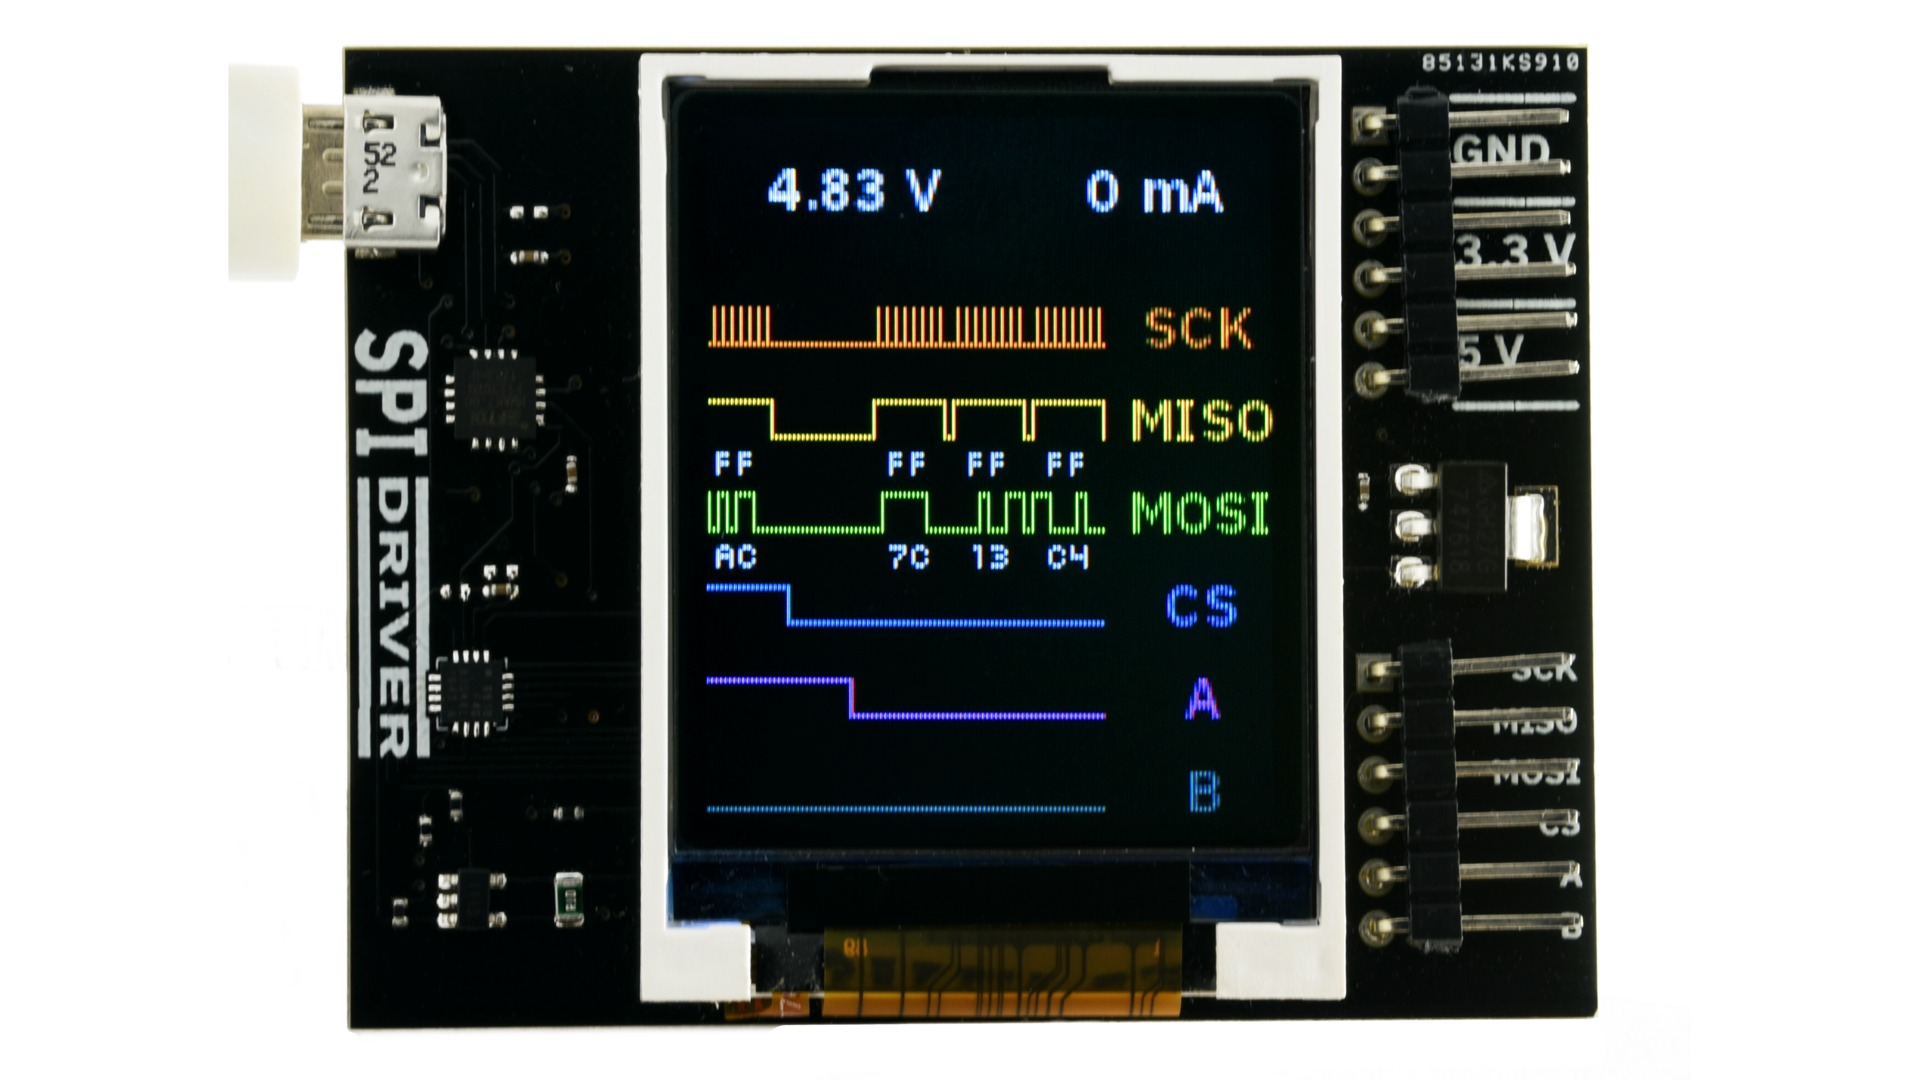
\includegraphics[width=1.00\textwidth]{img/spidriver/main}
Last updated on \today
\end{center}
\tableofcontents

\newpage

\setlength{\parindent}{0mm}
\setlength{\parskip}{1mm}
\setstretch{1.4}

\section{Overview}

SPIDriver is an easy-to-use tool for controlling SPI devices over USB.
It works with Windows, Mac, and Linux, and has a built-in color screen that shows a live logic-analyzer display of all SPI traffic.

\subsection{Features}
\begin{itemize}
\item live display shows you exactly what it’s doing all the time
\item sustained SPI transfers at 500 Kbps
\item USB line voltage monitor to detect supply problems, to 0.01 V
\item target device high-side current measurement, to 5 mA
\item two auxiliary output signals, A and B
\item dedicated power out lines. two each of GND, 3.3 V and 5 V
\item all signals color coded to match jumper colors
\item all signals are 3.3 V, and are 5 V tolerant
\item uses an FTDI USB serial adapter, and Silicon Labs automotive-grade EFM8 controller
\item also reports uptime, temperature, and running CRC of all traffic
\item all sensors and signals controlled using a simple serial protocol
\item GUI, command-line, C/C++, and Python 2/3 host software provided for Windows, Mac, and Linux
\end{itemize}

\newpage
\section{Getting Started}

When you first connect it to the USB port, the display blinks white for a moment then shows something like this:

\png{img/spidriver/spidriver-close}

Connect the six colored hookup jumpers as shown,
following the same sequence as on the screen

\gap
\begin{center}
\begin{tabular}{ll}
\hline
\mach{SCK}  & orange \\
\mach{MISO} & yellow \\
\mach{MOSI} & green  \\
\mach{CS}   & blue   \\
\mach{A}    & purple \\
\mach{B}    & gray   \\
\hline
\end{tabular}
\end{center}
\gap

The top six signals carry power. There are two each of GND, 3.3 V and 5 V.

Across the top of the display SPIDriver continuously measures the USB input voltage,
and the current output.

\newpage
\section{Software installation}

The source for all the SPIDriver software is the
\href{https://github.com/jamesbowman/spidriver}{repository}.
Available are:

\begin{itemize}
\item a Windows/Mac/Linux GUI
\item a Windows/Mac/Linux command-line
\item Python 2 and 3 bindings
\item Windows/Mac/Linux C/C++ bindings
\end{itemize}

Installation of the GUI and command-line utilities varies by platform.

\subsection{Windows}\index{software!Windows}

This
\href{https://spidriver.com/windows}{installer}
contains the GUI and command-line utilities.
The GUI shortcut is installed on the desktop:

\png{img/spidriver/icon}

launching it brings up the control window:

\png{img/spidriver/gui}

If there is only one serial device, 
the SPIDriver device should be automatically selected.
If there is more than one device, select its COM port from the pulldown menu at the top.
Once connected, you can control the signal lines and transmit hex values.

\index{spicl@\mach{spicl}}
The command line utility \mach{spicl} is also installed. For example to display status information:

\begin{lstlisting}
  C:\>"c:\Program Files\Excamera Labs\SPIDriver\spicl.exe" COM3 i
  uptime 1625  4.810 V  45 mA  23.3 C
\end{lstlisting}

See below for more information on the command-line syntax.

\subsection{Linux}\index{software!Linux}

The Linux GUI is available for download as
\href{https://spidriver.com/linux}{spigui-linux64}.
Alternatively you can run the native Python GUI directly as shown below.

\index{spicl@\mach{spicl}}
To build the command-line tool, clone the
\href{https://github.com/jamesbowman/spidriver}{repository}, then do:
\begin{lstlisting}
    $ cd spidriver/c
    $ make -f linux/Makefile
    $ ./build/spicl /dev/ttyUSB0 i
\end{lstlisting}
and you should see something like:

\begin{lstlisting}
    uptime 2285  4.812 V  45 mA  23.6 C
\end{lstlisting}

\subsection{MacOS}\index{software!Mac}

The MacOS GUI is available for download as
\href{https://spidriver.com/mac}{spigui-macos}.
This is a Mac executable, so after downloading it do:
\begin{lstlisting}
    $ cd Downloads
    $ chmod a+x spigui-macos
    $ ./spigui-macos
\end{lstlisting}

Alternatively you can run the native Python GUI directly as shown below.

\index{spicl@\mach{spicl}}
To  build the command-line tool, clone the
\href{https://github.com/jamesbowman/spidriver}{repository}, then do:

\begin{lstlisting}
    cd spidriver/c
    make -f linux/Makefile
    ./build/spicl /dev/cu.usbserial-DO00QS8D i
\end{lstlisting}

(substituting your actual SPIDriver's ID for \mach{DO00QS8D})
and you should see something like:
\begin{lstlisting}
    uptime 2285  4.812 V  45 mA  23.6 C
\end{lstlisting}

Note that the port to use is \mach{/dev/cu.usbserial-XXXXXXXX}, as explained
\href{https://pbxbook.com/other/mac-tty.html}{here}.

\section{APIs}
\subsection{Python 2 and 3}

The SPIDriver bindings can be installed with \mach{pip} like this:

\begin{lstlisting}
    pip install spidriver
\end{lstlisting}

then from Python you can do:

\begin{lstlisting}
    >>> from spidriver import SPIDriver
    >>> s = SPIDriver("/dev/ttyUSB0") # change for your port
    >>> s.sel()                       # start command
    >>> s.write([0x9f])               # command 9F is READ JEDEC ID 
    >>> list(s.read(3))               # read next 3 bytes
    [239, 64, 24]
    >>> s.unsel()                     # end command
    >>>
\end{lstlisting}

and you should see something like:

\png{img/spidriver/spidriver-flash}

The GUI (which uses wxPython) can be run with:

\begin{lstlisting}
    python spigui.py
\end{lstlisting}

which depending on your distribution looks something like this:

\png{img/spidriver/spidriver-gui-linux}

There are more examples in the 
\href{https://github.com/jamesbowman/spidriver/tree/master/python/samples}{\mach{python/samples}} folder in the repository.

\subsection{C/C++}

SPIDriver is contained in a single source file with a single header.
Both are in the
\href{https://github.com/jamesbowman/spidriver/tree/master/c/common}{\mach{c/common}} folder in the repository.
Usage follows the Python API and is fairly self-explanatory.

\newpage
\section{Using SPIDriver}

\subsection{The command-line tool \mach{spicl}}
\index{spicl@\mach{spicl}}

\mach{spicl} is the same on all platforms.

The first parameter to the command is the serial port, which depends on your operating system.
All following parameters are control commands. These are:

\gap\begin{tabular}{ll}
\hline \\
  \mach{i}     & print status information (uptime, voltage, current, temperature) \\
  \mach{s}     & SPI select \\
  \mach{u}     & SPI unselect \\
  \mach{w} $byte$\mach{,}...     & write bytes to SPI \\
  \mach{r N}   & read N bytes from SPI \\
  \mach{a 0/1} & Set A line \\
  \mach{b 0/1} & Set B line \\
\hline \\
\end{tabular}
\gap

For example the command:

\begin{lstlisting}
  spicl /dev/ttyUSB0 s w 0x9f r 3 u
\end{lstlisting}

does the following:

\gap\begin{tabular}{ll}
\hline \\
 \mach{s}       & SPI select \\
 \mach{w 0x9f}  & Write byte \mach{0x9f} \\
 \mach{r 3}     & Read 3 bytes from slave \\
 \mach{u}       & SPI unselect \\
\hline \\
\end{tabular}

Byte values are decimal by default, or hex if prefixed with \mach{0x}.
To send multiple bytes, separate them with a comma.

\section{Examples}
\subsection{ST7735R 1.8" LCD}\index{Examples!ST7735R}

The ST7735R is a small color LCD controller,
with a panel resolution of 160x128.
It has an SPI-like interface. It does not use MISO, and needs an
extra control line to distinguish between command bytes and data bytes.
It requires an external reset for reliable start-up.

Connect the LCD panel like this:

\pngw{img/spidriver/spidriver-lcd-1}{0.5}

\begin{center}
\gap\begin{tabular}{ccc}
\hline
SPIDriver&        & LCD     \\
\hline
3.3V     & brown  & LED     \\
SCK      & orange & SCK     \\
MOSI     & green  & SDA     \\
A        & purple & A0      \\
B        & gray   & RESET   \\
CS       & blue   & CS      \\
GND      & black  & GND     \\
3.3V     & red    & VCC     \\
\hline \\
\end{tabular}
\end{center}


There is a Python demonstration program for loading images onto the display.
It requires pillow for image loading, so you may need to install its prerequisites:

\begin{lstlisting}
    pip install pillow
\end{lstlisting}

Then in the SPIDriver repository do:

\begin{lstlisting}
    cd python/samples
    python st7735s.py -h /dev/ttyUSB0 grace.png
\end{lstlisting}

You can supply any image files as the last argument,
and the script will resize and display them in order.

\subsection{SPI Flash}\index{Examples!SPI flash}\index{flash}

First confirm the flash pinout on its datasheet. Modern SPI flash chips have a pinout like this one:

\png{img/spidriver/spidriver-flash-0}

Connect the clip to the flash, oriented with the red cable on pin 1.
For example this is the clip connected to the flash on a ESP8266 board:

\png{img/spidriver/spidriver-esp1}
 
\index{ESP8266}
For the ESP8266, the CPU needs to be kept in reset so there is no contention while SPIDriver is driving to the flash.
Connect SPIDriver's A signal (purple) to the ESP8266 reset:
 
\png{img/spidriver/spidriver-esp2}

\png{img/spidriver/spidriver-flash-2}

and connect the clip cable pins to the SPIDriver like this:

\begin{center}
\gap\begin{tabular}{ccc}
\hline
SPIDriver&        & flash   \\
\hline
\mach{CS}         & blue   & 1 \\
\mach{MISO}       & yellow & 2 \\
                  &        & 3 \\
\mach{GND}        & black  & 4 \\
\mach{MOSI}       & green  & 5 \\
\mach{SCK}        & orange & 6 \\
                  &        & 7 \\
\mach{3.3V}       & red    & 8 \\
\hline \\
\end{tabular}
\end{center}

\index{JEDEC ID}
You should be able to use the command-line utility to confirm the flash 3-byte JEDEC ID.
For example:

\begin{lstlisting}
    $ spicl /dev/ttyUSB0 a 0 u s w 0x9f r 3 u
    0xc8,0x40,0x13
\end{lstlisting}

The specific ID codes vary by manufacturer, and are listed in the datasheet for each flash part.
The third byte is the flash size in bits, so the flash above is
$2^{19} = 524288$ bytes, or 512K bytes.
If you don't see a valid ID, and you've checked the pinout,
make sure that the clip is properly making contact with all of the flash pins.

There is a Python example
\href{https://github.com/jamesbowman/spidriver/blob/master/python/samples/flash.py>}{flash.py}
that can read and write flash contents using standard
SPI flash commands.
With no options, it prints out JEDEC ID as confirmation:

\begin{lstlisting}
    $ python flash.py -h /dev/ttyUSB0
    Got JEDEC ID: c8 40 13
    Flash size is 524288 bytes
\end{lstlisting}

You can read all of flash into a file with the \mach{-r} option:

\begin{lstlisting}
    $ python flash.py -h /dev/ttyUSB0 -r flashfile
    Got JEDEC ID: c8 40 13
    Flash size is 524288 bytes
    0/512 KBytes
    8/512 KBytes
    ...
    504/512 KBytes
\end{lstlisting}

Similarly the \mach{-w} option erases the flash and writes a file to it:

\begin{lstlisting}
    $ python flash.py -h /dev/ttyUSB0 -w flashfile
    Got JEDEC ID: c8 40 13
    Flash size is 524288 bytes
    0/512 KBytes
    ...
    504/512 KBytes
\end{lstlisting}

Many flash devices -- like the one above -- report their size in bits in the third ID byte.
However some do not follow this convention.
To support these devices, the script's
\mach{-s} option specifies the device size in bytes, overriding the default calculation.

% The Shield Adapter
% ------------------
% 
% The shield adapter connects the SPIDriver signals to the Arduino's standard SPI locations,
% so you can use Arduino shields with the SPIDriver.
% In addition to power (GND, 3.3 V and 5 V) it connects:
% 
% ========= ===========
% SPIDriver Arduino Pin
% ========= ===========
% SCK       13
% MISO      12
% MOSI      11
% CS        8
% A         9
% B         10
% ========= ===========

\newpage
\section{Technical notes}

\subsection{Port names}\index{USB ports}\index{port names}

The serial port that SPIDriver appears at depends on your operating system.

On \textbf{Windows}, it appears as COM1, COM2, COM3 etc.
You can use the Device Manager or the \mach{MODE} command to display the available ports.
\href{https://plugable.com/2011/07/04/how-to-change-the-com-port-for-a-usb-serial-adapter-on-windows-7/}{This article}
describes how to set a device to a fixed port.

On \textbf{Linux}, it appears as \mach{/dev/ttyUSB0}, 1, 2 etc.
The actual number depends on the order that devices were added.
However it also appears as something like:
\begin{lstlisting}
    /dev/serial/by-id/usb-FTDI_FT230X_Basic_UART_DO00QS8D-if00-port0
\end{lstlisting}
Where \mach{DO00QS8D} is the serial code of the SPIDriver (which is printed on the bottom of each SPIDriver).
This is longer, of course, but always the same for a given device.

Similarly on \textbf{Mac OS}, the SPIDriver appears as \mach{/dev/cu.usbserial-DO00QS8D}.

\subsection{Decreasing the USB latency timer}

SPIDriver performance can be increased by setting the USB latency timer to its minimum value of 1 ms.
This can increase the speed of two-way SPI traffic by up to 10X.

On \textbf{Linux} do:

\begin{lstlisting}
    setserial /dev/ttyUSB0 low_latency
\end{lstlisting}

On \textbf{Windows} and \textbf{Mac OS} follow
\href{https://projectgus.com/2011/10/notes-on-ftdi-latency-with-arduino/}{these instructions}.

\subsection{Temperature sensor}\index{temperature sensor}

The temperature sensor is located in the on-board EFM8 microcontroller.
It is calibrated at manufacture to within 2 C.
A sudden temperature rise may indicate that one of the output pins (MOSI, SCK, CS, A, or B) is shorted to VCC or GND.

\subsection{Raw protocol}\index{protocol}

SPIDriver uses a serial protocol to send and receive SPI commands.
Connect to the SPIDriver at 460800 baud, 8 bits, no parity, 1 stop bit (460800 8N1).
\index{speed!serial}
Many SPIDriver commands are ASCII, you can control it
interactively from any terminal application that can connect at 460800
baud. For example typing u and s toggles the CS line and ? displays the
status info.
Commands are:

\gap\begin{tabular}{ll}
\hline
\mach{?}        & transmit status information (see below)        \\
\mach{e} $byte$ & echo $byte$       \\
\mach{s}        & select        \\
\mach{u}        & unselect        \\
\mach{a} $byte$ & set A output to 0/1       \\
\mach{b} $byte$ & set B output to 0/1       \\
\mach{x}        & disconnect from SPI bus       \\
\mach{0x80-bf}  & write and read 1-64 bytes       \\
\mach{0xc0-ff}  & write 1-64 bytes        \\ \hline
\end{tabular}\gap

So for example to select, transfer two bytes
\mach{0x12,0x34},
unselect, the host sends 5 bytes.
The command \mach{0x81} is a two byte send/receive, so two bytes are returned to the PC.

\begin{lstlisting}
s
0x81
0x12
0x34
u
\end{lstlisting}


The status information is always 80 characters, space padded. For example:

{\scriptsize
\begin{framed}\begin{Verbatim}
[spidriver1 DO00QS8D 000007219 4.807 045 25.4 1 1 1 49c1                       ]
\end{Verbatim}
\end{framed}}

The fields are space-delimited:

\gap\begin{tabular}{ll}
\hline
spidriver1      & fixed identifier \\
serial          & serial code identifier \\
uptime          & SPIDriver uptime 0-999999999, in seconds \\
voltage         & USB bus voltage, in volts \\
current         & attached device current, in mA \\
temperature     & junction temperature, in C \\
CS              & CS line state \\
A               & A line state \\
B               & B line state \\
crc             & 16-bit CRC of all input and output bytes (CRC-16-CCITT)  \index{CRC}\\
\hline
\end{tabular}\gap

\newpage
\subsection{Specifications}\label{electrical-characteristics}

\subsubsection*{DC characteristics}
\vspace{10 pt}
{\renewcommand{\arraystretch}{1.2}% for the vertical padding

\begin{tabularx}{\linewidth}{XC{40pt}C{40pt}C{40pt}C{40pt}}
\heavyline
& min & typ & max & units \\ \heavyline

Voltage accuracy              && 0.01 && V            \\ \hline
Current accuracy              && 5 && mA              \\ \hline
Temperature accuracy          && $\pm$ 2 && $^{\circ}$C            \\ \hline
MISO & & & & \\
\hspace{10pt}low voltage & & & 0.6 & V \\
\hspace{10pt}high voltage & 2.7 &   & 5.8 & V \\ \hline
Output signal current (SCK, MOSI, CS, A, B)  &&& 8 & mA \\ \hline
Output current        & & & 470 & mA                  \\ \hline
Current consumption   & & 25 & & mA                   \\ \hline

\end{tabularx}}
\vspace{10 pt}

\subsubsection*{AC characteristics}
\vspace{10 pt}

{\renewcommand{\arraystretch}{1.2}% for the vertical padding
\begin{tabularx}{\linewidth}{XC{40pt}C{40pt}C{40pt}C{40pt}}
\heavyline
& min & typ & max & units \\ \heavyline

SPI speed                     &495& 500 &505& Kbps   \index{speed!SPI}\\ \hline
Uptime accuracy               && 150 && ppm           \index{uptime}\\ \hline
Uptime rollover               && 31.7 && years        \\ \hline
Startup time & & & 200 & ms \\ \hline
\end{tabularx}}
\vspace{10 pt}

\section{Support information}

Technical and product support is available at
\href{mailto:support@spidriver.com}{support@spidriver.com}

SPIDriver is built and maintained by
\href{https://excamera.com}{Excamera Labs}.

\newpage
\raggedright
\addcontentsline{toc}{section}{Index}
\renewcommand{\indexname}{Index}
\printindex

\end{document}
